\chapter{绪论}
\section{研究背景}
\textit{Stacker.}\linkout{stacker}{1}
\textit{Tiered Storage Systems}:\linkout{Adaptive_Data_Migration_in_Multi-tiered_Storage_Based_Cloud_Environment}{1}
\subsubsection*{分层存储技术}
分层存储系统(Tiered Storage System),又称为层级存储管理(Hierarchical Storage Management),是当前各领域存储系统的主流架构。其基本特点是将文件数据存储在若干层级的存储介质中,不同层级的介质(DRAM,SSD,HDD等)具有不同的容量、吞吐率、访问延迟与成本等。不同的应用负载和场景下,存储系统中的数据重要性存在差异,可以粗略地分为“热”数据与“冷”数据:正在访问与频繁访问的“热”数据优先存储于更接近CPU、访问更快的内存、SSD阵列等存储介质中;近期没有访问需求或访问频率低的“冷”数据主要存储在低层级的磁盘阵列或远程存储服务器中。在现实应用中,数据的“热”与“冷”不是静态的,而是随着应用的访问需求动态变化,数据在不同层级之间的迁移管理成为层次存储系统的基本任务之一。
\begin{figure}[htp]
    \centering
    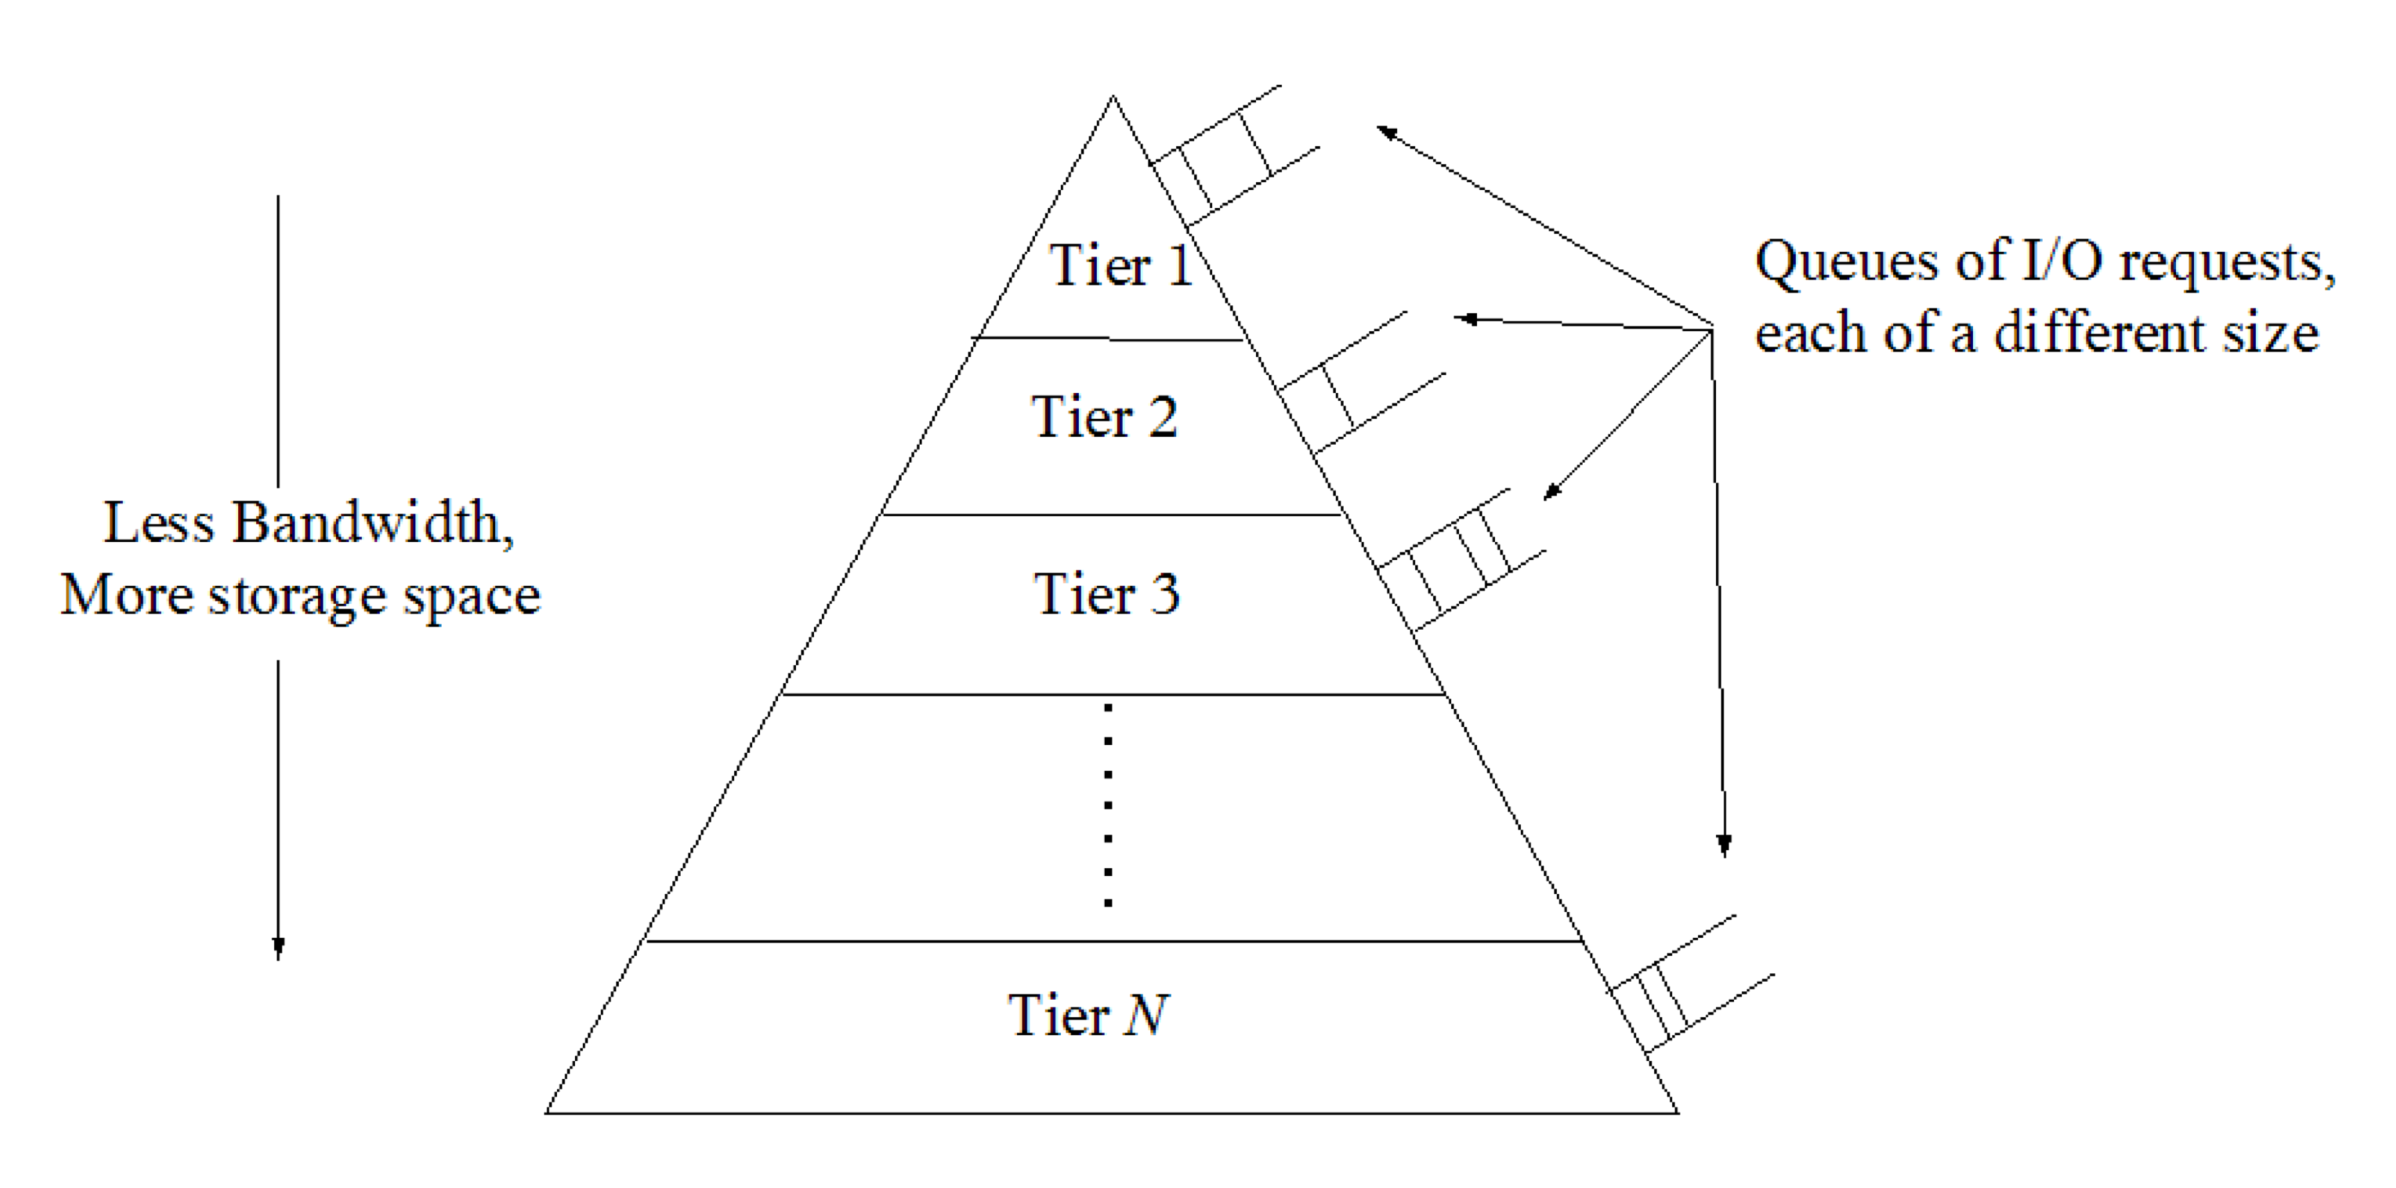
\includegraphics[width=\textwidth]{chp2_multi_tiers}
    \caption{分层存储系统(Tiered Storage System)}
    \label{fig:multi_tiers}
\end{figure}
如图\ref{fig:multi_tiers}所示,分层存储系统按层级从高到低由不同存储介质组成:
\begin{itemize}
    \item 高层级存储通常由内存DRAM(Dynamic Random Access Memory)、非易失性存储(Non-volatile Memory)等介质组成,其特点是读写性能优异、存储密度高,是实际应用场景中“热”数据的理想存储载体,同时也具有易失(DRAM)或寿命有限(NVM)等缺点
    \item 较低级存储通常由固态硬盘(Solid-State Driver)、磁盘(Hard Disk Drive)阵列组成,且在生产环境下这些存储阵列通常部署在远程存储服务器(Storage Servers),通过SANs(Storage Area Networks)或高速互联网络(InfiniBand)与客户端或计算服务器连接以提供存储服务。低层级存储性能较弱,存储密度较低,但同时也具有造价低廉、容量大、稳定性好的优点,且可以通过冗余磁盘阵列(Redundant Array of Inexpensive Disks)以及数据复制(Replication)等技术进一步提高数据的稳定性和容错能力。因此这类低层级存储是“冷”数据的理想载体。
\end{itemize}


近几十年来,分层存储在商业性数据存储领域得到了大规模应用。例如NetApp FAS系列存储系统
\cite{NetAppFas},
IBM DS8880
\cite{IBMDS8880}
等。这些支持Flash存储介质的存储系统方案主要可分为两类:第一类存储方案简单地将Flash存储介质作为较内存低一级的缓存
\cite{NetAppFas}
,以起到优化存储系统性能的作用。采用Flash存储介质作为缓存的主要优点是集成容易,不需要显式地考虑数据迁移策略,同时造价比DRAM低得多。第二类方案则是将Flash存储介质作为持续存储加入到层次存储结构中。

在大规模科学与工程计算领域,层次存储结构同样应用广泛。随着闪存技术的飞速发展,传统HPC所应用的三层技术架构(计算结点的共享内存-并行文件系统-归档存储)也随之发生变化。在HPC系统中,并行文件系统(pFS)对HPC性能影响非常大,在许多场景下决定了整个HPC的存储性能。传统HPC架构在应对超大规模HPC集群计算节点同时Checking Point需求时,显得力不从心,那就需要在pFS之上多加一层高速大容量(相对于Memory)的缓存(Burst Buffer)。典型代表有
{\color{red}此处补充采用Burst Buffer技术的超算架构}

\subsubsection*{分层存储架构中的数据迁移管理}
层次存储系统中的不同层级间的数据迁移管理是文件系统性能的关键。可粗略分为被动缓存和主动预取。预取(prefetching),也称为预分页(prepaging)或预读(read-ahead),是操作系统数据读取过程中的重要优化方法
\cite{Reducing_File_System_Latency_using_a_Predictive_Approach}
\cite{Group_based_management_of_distributed_file_caches}
\cite{A_data_mining_algorithm_for_generalized_web_prefetching}
。其目标是预测将来的数据访问,并在请求数据之前将其提前读取到高层级的存储介质中,从而起到掩盖访问延迟的作用。预取是传统缓存技术的一种补充,不同于被动数据迁移,预取技术的关键在于对即将访问的数据内容和生存周期进行主动预测。

\begin{itemize}
\item \textbf{“热”数据预测}:主动预取需要预测程序下一阶段可能访问的数据,是对数据访问的空间局部性的扩充。针对“热”数据准确的预测将极大地降低访问延迟,而错误预测将会引发浪费传输带宽,挤占缓存空间等负面影响。
\item \textbf{“热”数据生命周期预测}:与缓存机制中的时间局部性类似,主动预取需要针对缓存数据的时效性和生命周期建立有效的评估。非缓存数据的及时预取有助于提高存命中率,而清除短期内不再读取的数据将提高缓存空间的利用率。
\end{itemize}

预取的主要流程可总结如下:
\begin{enumerate}
\item 针对特定负载,提取访问日志;
\item 分析访问日志,对该负载的文件访问模式进行抽象表达;
\item 将负载的访问模式作为依据,引导文件系统进行主动预取。
\end{enumerate}

{\color{red}缓存vs预取概念对比图}

\section{国内外研究现状}
%\linkout{overview}{14}
Eshel等\cite{Panache}
提出并实现了缓存文件系统“Panache”,该系统使用pNFS以分布式缓存的方式存储GPFS中的缓存数据。
Frings等\cite{Massively_Parallel_Loading}
针对动态链接库加载过程进行数据预取,从而提高并行应用程序的性能。
Rajachandrasekar等\cite{1PB}
提出了一种用户级文件系统,将检查点请求保留在主内存中,并同时写入到持久性存储中。他们的方法包括对远程直接内存访问(RDMA)的支持。

Zhao等\cite{HyCache+}
提出了另一种缓存中间件,采用一种双阶段缓存技术来减少计算结点和I/O结点之间的数据传输量。
Isaila等\cite{Multi_Leve_Data_Staging_for_Blue_Gene}
提出了分别位于客户端和I/O节点之间,以及I/O节点和存储服务器之间的两级预取方案,从而改进了IBM Blue Gene的I/O转发层的数据传输性能。
Prabhakar等\cite{Adaptive_Multi_level_Cache_Allocation_in_Distribute_Storage_Architectures}
通过线性规划对两级缓存系统上的最佳缓存分配进行建模。

Kandemir等\cite{On_Urgency_of_I/O_Operations}
定义了I/O请求紧迫度的概念,该概念由请求可以延迟多长时间而不影响应用程序性能给出。在对I/O请求进行紧迫度分析后,通过优先处理紧急请求来改进缓存机制。
Seelam等\cite{Masking_IO_latency_using_application_level_IO_caching_and_prefetching_on_Blue_Gene_systems}
实现了能够追踪和分析应用I/O访问模式的库,并借此引导预取线程将数据提前读取到本地存储。
Patrick\cite{Cashing_in_on_Hints_for_Better_Prefetching_and_Caching_in_PVFS_and_MPI_IO},
He\cite{KNOWAC},
Tang\cite{Improving_read_performance_with_online_access_pattern_analysis_and_prefetching}
等提出了类似的方法(使用访问模式检测指导预取)。


Suei等\cite{Endurance_Aware_Flash_Cache_Management_for_Storage_Servers}
提出了一种使用SSD作为HDD缓存的存储集群缓存设计。其设计侧重于响应时间和缓存命中率。 

Welch和Noer\cite{Optimizing_a_hybrid_SSD_HDD_HPC_storage_system_based_on_file_size_distributions}
根据并行文件系统中小文件占多数的特点,将小文件存储在SSD中以优化对它们的访问。
He等\cite{Proceedings_of_the_22nd_international_symposium_on_High_performance_parallel_and_distributed_computing}
提出了一个代价模型来辅助数据迁移决策。该模型能够评估文件不同区域的访问成本,并将高成本区域放置在SSD中。

\section{本文主要工作}
\begin{itemize}
    \item 研究分析GlusterFS的原理、架构和功能实现,提出基于Tiering模块的数据迁移管理框架设计。
    \item 针对POSIX文件系统的目录结构、命名习惯等特点,提出采用词向量模型进行量化分析,即,将文件或目录映射到高维向量空间来分析文件、目录间的逻辑关系。
    \item 针对特定工作负载的I/O访问模式进行研究,在文件/目录向量化工作的基础上,采用循环神经网络提取和分析I/O访问模式,并用于替代传统的缓存算法(LRU等)指导GlusterFS进行数据迁移。
\end{itemize}
\section{论文结构}